% vim:encoding=utf8 ft=tex sts=2 sw=2 et:
% Copyright (c) 2009 Jaroslaw Koszuk
%
% $Id$

\documentclass{jacsart}

\usepackage[utf8]{inputenc}
\usepackage[T1]{fontenc}
\usepackage{graphicx}
\usepackage{amsthm}
\usepackage{txfonts}
\usepackage{hyperref}


\newtheorem{definition}{Definition}
\newtheorem{theorem}[definition]{Theorem}
\newtheorem{corollary}[definition]{Corollary}
\newtheorem{proposition}[definition]{Proposition}
\newtheorem{example}[definition]{Example}


\title{Natural User Interfaces (NUI): Review}
\headtitle{Natural User Interfaces (NUI): Review}
\author{Grzegorz Glonek\inst{1}, Maria Pietruszka\inst{2}}
\headauthor{G. Glonek, M. Pietruszka}
\affiliation{%
  \inst{1}Łódź University of Technology\\
  Institute of Information Technology\\
  Wólczańska 215, 90-924 Łódź, Poland\\
  grzegorz@glonek.net.pl
  \andinst
  \inst{2}Łódź University of Technology\\
    Institute of Information Technology\\
    Wólczańska 215, 90-924 Łódź, Poland\\
    maria.pietruszka@p.lodz.pl}
\keywords{gestures, touch, natural user interfaces, Kinect, Move, Wii}

\begin{document}
\maketitle

\begin{abstract}
The article summarizes and systematizes knowledge concerning natural user interfaces. The most important facts related to this problem have been supplemented with examples of possible practical use of such type of human-computer communication. Moreover, the article contains descriptions of three most popular controllers: Microsoft Kinect, Nintendo Wii and Sony Move. 
\end{abstract}

\section{Introduction}
\indent Natural User Interfaces (NUI) were created in an attempt to establish new ways of communication between human beings and machines (computers in particular). As far as the analysis of human-computer interactions is concerned, NUI is one of four types of User Interfaces (UI) \cite{Liu2010b}, including Batch Interface (BI), Command Line Interface (CLI) and Graphical User Interface (GUI).\\
\indent Although the very term NUI has become increasingly popular after 2006, when Jefferson Hen on TED conference presented the results of his research on multi-touch interfaces \cite{Han2006}, research concerning this subject had already been conducted in the 1990s \cite{Rauterberg1997, Rauterberg1996, Rauterberg1996a}. However, the unquestionable forerunner of research in the field of alternative ways of interaction with computer systems and at the same time the person who coined the name NUI was Prof. Steve Mann from Toronto University, who started conducting research on interaction with computer with the use of virtual reality in the early 1980s.\\
\indent Term NUI stands for the ways of interaction with a device based on methods other than a mouse and a keyboard that would at the same time be as natural and intuitive for a human being as possible. Therefore, such interfaces can be based e.g. on voice, touch or image and movement detection and interpretation. Such devices as Nintendo Wii, Sony Move or Microsoft Kinect together with dedicated games are the most popular adaptations of the NUI idea. All of them are based on movement detection, however, they realize it in various ways. Nintendo Wii and Sony Move require the player to use devices which serve as different kinds of tags, while Kinect recognizes player’s body parts and tracks their movement. Additionally, Kinect is able to recognize voice commands.\\
\indent Next chapter describes these three game devices and way they work.  Following chapters contains information about usage of NUI (chapter \ref{sec:use}), direction of development and research centers (chapters \ref{sec:development} and \ref{sec:centers}) and criticism of this way of communication.

\section{Movement controllers} \label{sec:controllers}
\subsection{Nintendo Wii Remote} \label{ssec:wiimote}

\indent Wii Remote controller (Wiimote) is a basic input interface for Nintendo Wii console. It has been constructed as a wireless device, at whose ''heart'' is an integrated circuit Broadcom BCM 2042, which communicates by means of Bluetooth technology \cite{wiibrew}. Moreover, the controller is equipped with accelerometer (integrated circuit ADXL330), which allows for determining movement in three planes x, y and z. Wiimote makes it also possible to determine one’s own rotation  with respect to each of the mentioned axes (Fig. \ref{fig:wiimote}).\\
\indent The last frame of reference which may be used by the creators of applications using Nintendo Wii Remote is the distance between the controller and the device called Sensor Bar. Sensor Bar (Fig. \ref{fig:WiimoteSensorBar}) is a device equipped with a sequence of diodes in the infrared band with a known distance between each diode. Thanks to that information and the image recorded by a camera with infrared filter which is built in the controller, it is possible to determine the distance between the Sensor Bar and the user. The distance is calculated as follows:

\begin{figure}[!t]
\centering
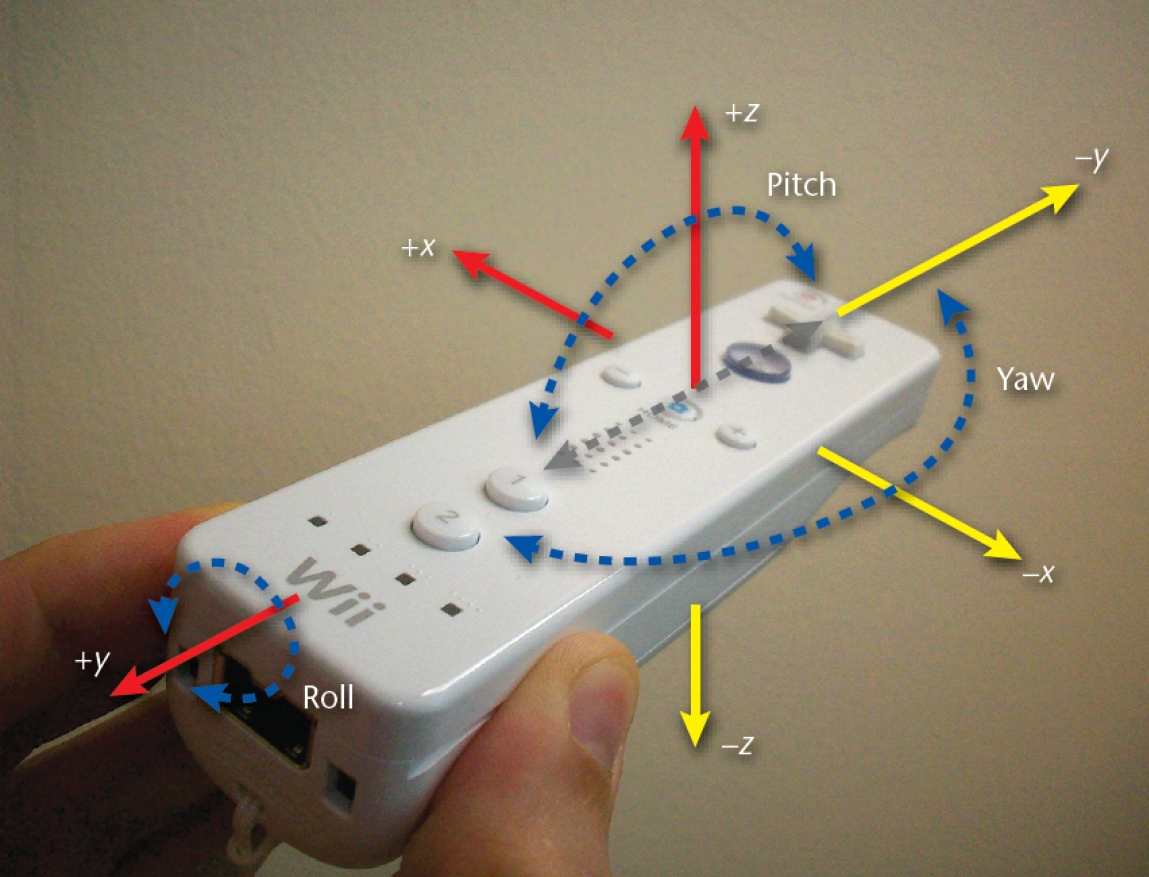
\includegraphics[width=0.9\textwidth]{WiiMoteCoordinates.jpg}
\caption{Wiimote – frames of reference x, y and z and rotations with respect to each of these axes \cite{Jr2011}.}
\label{fig:wiimote}
\end{figure}

\begin{equation}d = \sqrt{{d_L}^2 + (m/2)^2 - 2d_L(m/2)^2\cos{\phi}}\end{equation}

\begin{equation}\cos{\phi} = \frac{{d_L}^2m^2 - {d_R}^2}{2md_L}\end{equation}

\begin{equation}d_L = \frac{w_L/2}{\tan{\phi/2}}\end{equation}

\begin{equation}d_R = \frac{w_R/2}{\tan{\phi/2}}\end{equation}

\begin{equation}w_L = \frac{w_{img} \mathit{diam}_{LED}}{\mathit{diam}_L}\end{equation}

\begin{equation}w_R = \frac{w_{img} \mathit{diam}_{LED}}{\mathit{diam}_R}\end{equation}

where:
\begin{itemize}
\item{$d$ – the distance between the user and Sensor Bar}
\item{$m$ – the distance between the right and the left diode in Sensor Bar}
\item{$w_{img}$ – the width of the image recorded by the controller’s camera}
\item{${diam}_{LED}$ – the actual diameter of the Sensor Bar diode}
\item{${diam}_L$ – the diameter of the left diode on the camera image}
\item{${diam}_R$ – the diameter of the right diode on the camera image }
\end{itemize}

\begin{figure}[!t]
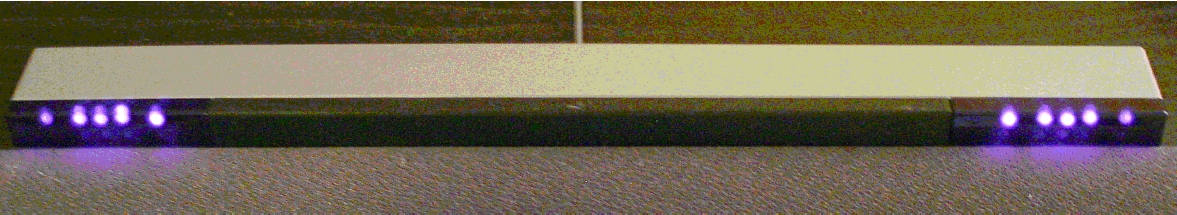
\includegraphics[width=0.9\textwidth]{NintendoSensorBar}
\caption{Nintendo Sensor Bar \cite{Jr2011}.}
\label{fig:WiimoteSensorBar}
\end{figure}

\subsection{Sony Move} \label{ssec:move}

\indent The system created by Sony consists of a camera called PlayStation Eye and max. 4 Sony Move controllers (Fig. \ref{fig:moveControler}).

\begin{figure}[!t]
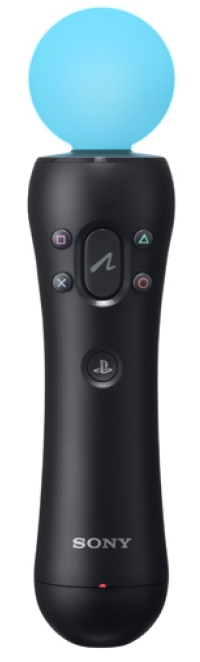
\includegraphics[angle=90, width=0.9\textwidth]{SonyMove.jpg}
\caption{Sony Move Controller \cite{Jr2011}.}
\label{fig:moveControler}
\end{figure}

\indent The controller is based on 3 gyroscopes and 3 accelerometers which allows for determining the inclination towards each axis as well as the movement along them. The other element of the system, i.e. PlayStation Eye, cooperates with more than a four-centimetre sphere at the end of the controller. It helps to determine the spatial location of the controller (and, at the same time, the user). Thanks to that, a spherical shape of a given color is being detected on the image from the camera, which is quite simple. Such approach allows for simple and precise tracking of the users in rooms with insufficient amount of light. Owing to the fact that the size of the sphere on the controller is known and the parameters of the camera lens are constant, it is possible to determine the distance between the player and the device. Figure \ref{fig:moveResults} shows the result of controller detection on the image registered by PlayStation Eye.\\
\indent The way Sony Move works and the structure of the system is very similar to Wiimote and could be treated as a development and perfection of the Nintendo’s idea.\\

\begin{figure}[!t]
\centering
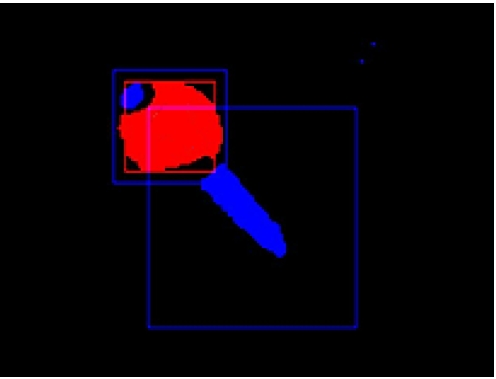
\includegraphics[width=0.5\linewidth]{SonyMoveCameraImage.jpg}
\caption{The result of controller detection on the image registered by PlayStation Eye \cite{Jr2011}.}
\label{fig:moveResults}
\end{figure}

\subsection{Microsoft Kinect} \label{ssec:kinect}

\indent The most advanced controller which is at present available on the market is Microsoft Kinect, which appeared in shops between the previously described devices. The main assumption of its creators was to eliminate additional devices so that the player would use whole body to control the application. The device is able to recognize and track the movement of a few people at the same time as well as recognize their voice commands. The very device is of a rather small size and consists of traditional RGB camera of 640x480 resolution, distance detector, microphone and servomotor, whose task is to stabilize the position of the device and help in its calibration (Fig. \ref{fig:kinectOverview})\\

\begin{figure}[!t]
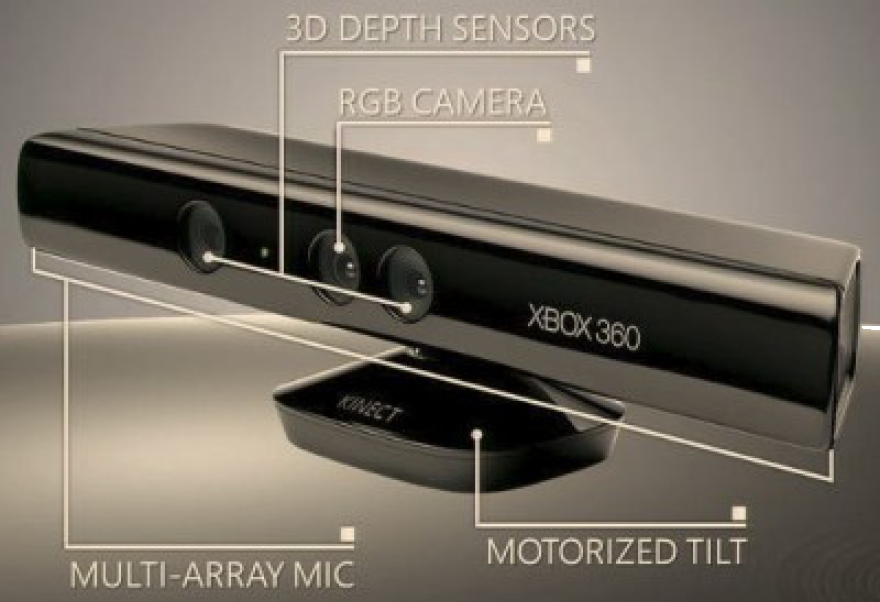
\includegraphics[width=0.9\linewidth]{./kinect}
\caption{Microsoft Kinect Controller \cite{Jr2011}.}
\label{fig:kinectOverview}
\end{figure} 

\indent RGB camera detects features of the user and the surroundings, especially the color of the clothes, the color of the surroundings and recognizes the user’s face. It is important as some applications which use this controller automatically log the users in to their accounts if only they are recognized, and their virtual avatar adjusts its clothes to match the present clothes of the user. The microphone and the software are able to recognize voices of a few users at the same time and to distinguish them even in a noisy surrounding. It is very interesting that when the user is identified on the basis of his or her voice, the camera focuses only on the recognized person and is able to show only them plus maybe the people who are standing right next to them. It is a feature which is particularly practical in the case of applications allowing for teleconferences since the attention can be focused only on the speaker and not on all the people in the room. Similarly to Nintendo Wiimote and Sony Move, Kinect provides the information about the distance between the user and the device.\\
\indent The fact that the user does not have any other tags but his own body forced the creators to come up with a totally new way of operating which differs from their competitors’. The infrared projector emits a lot of infrared beams all over the room and marks them as dots as shown in figure \ref{fig:kinectDots}. Next, CMOS\footnote{CMOS -- complimentary metal-oxide semiconductor}  matrix is able to locate these dots in space. The data collected by the matrix are later on processed by the software.\\

\begin{figure}[!t]
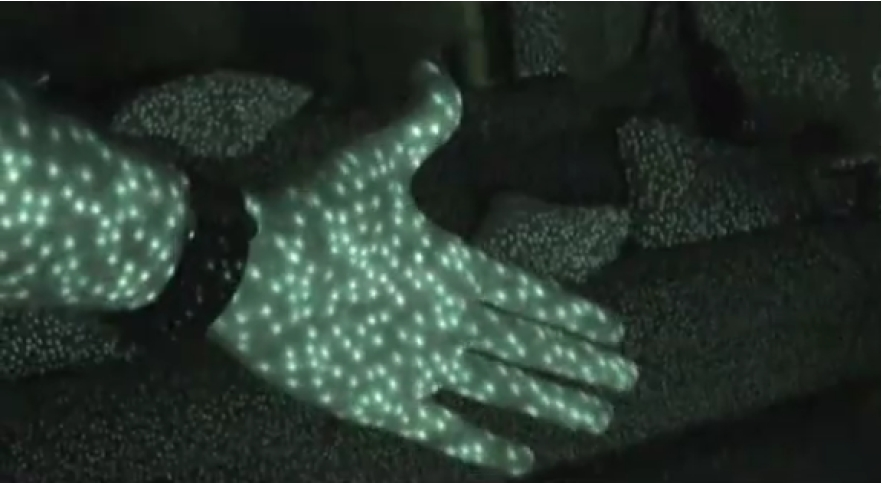
\includegraphics[width=0.9\linewidth]{./kinectIRLighting}
\caption{Marking the room with infrared beams by Microsoft Kinect \cite{Jr2011}.}
\label{fig:kinectDots}
\end{figure} 

\indent The information about the depth is determined on the basis of stereoscopic triangulation. In classic approach, this method requires images from two cameras in which points representing the same objects are detected.  In the next step the disparition between these images is determined, which allows for determining the distance by means of triangulation. In the case of Kinect this process is slightly different due to the lack of two cameras. The infrared projector determines the angles of the infrared light beams in a pseudorandom way. Such a pattern is treated as the first image required to run the above-mentioned process.  The second image is represented by the data collected from the CMOS matrix, i.e. the actual locations of the generated beams. Thanks to the data prepared this way, it is possible to create a depth map of the surrounding. Figure \ref{fig:kinectDepth} presents a sample map.\\
\indent Tracking multiple users at the same time is possible not only because of the processes described above but also by skeletonization\footnote{skeletonization – a process which allows for separating axis object points in the analyzed image or its fragment. Skeletonization changes the original image into a series of thin segments, arches and points called skeletons. Characteristic feature of a skeleton is the fact that it is always smaller than the object but retains all its topological features \cite{Radzienski2007}.}. In order to carry out this operation as precisely as possible, the data from all the sensors as well as the knowledge of the movements of human body collected by the engineers is used.\\
\indent Thanks to this feature, the device is insensitive to the situations in which the players switch places or when one of the players covers the other one. Figure \ref{fig:kinectSkeleton} shows the ''skeleton'' of a person using such a controller.\\

\begin{figure}[!t]
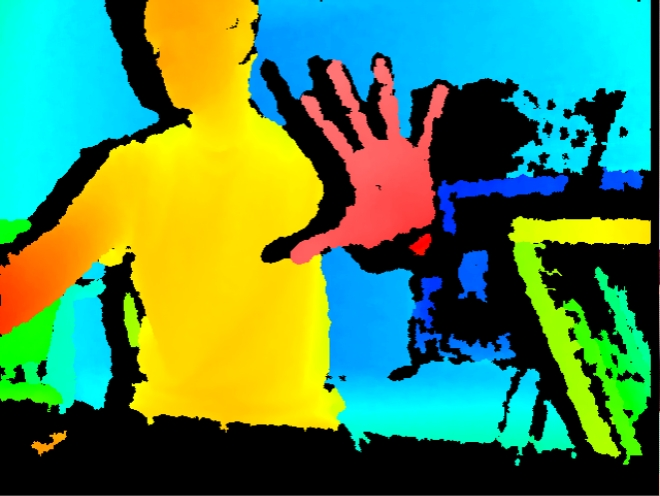
\includegraphics[width=0.9\linewidth]{./kinectDepthImage}
\caption{Sample depth map created by Microsoft Kinect \cite{Jr2011}.}
\label{fig:kinectDepth}
\end{figure} 

\indent All the calculations necessary for the device’s proper operation are done by components which are in it. Owing to that fact, a high efficiency of data processing could have been achieved. The most sensitive component of the device is the technology behind the creation of the depth map, which was devised by the Prime Sense Company. What is interesting, Prime Sense provides its technologies exclusively for Microsoft but so far this exclusiveness has concerned only the game consoles market. Microsoft Kinect was produced with a view to the game industry and was dedicated only to Xbox 360 console. However, the home creators quickly supplied the necessary libraries and drivers and the device was launched on PCs. Because of the ambiguous licensing Kinect on PCs was until recently used mainly by the enthusiasts, but now an official version of this device for PCs is available on the market.\\

 \begin{figure}[!t]
 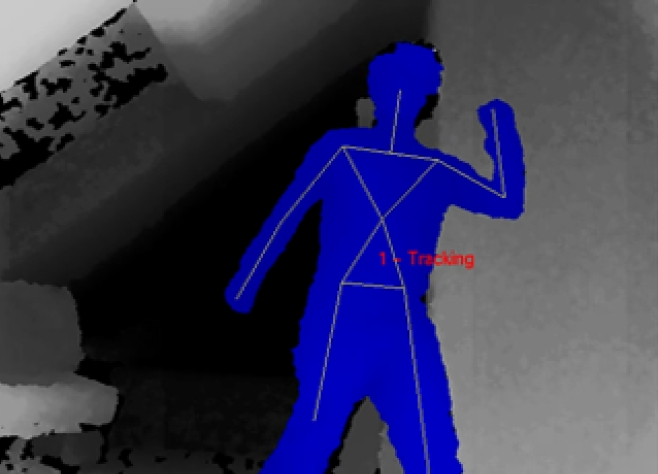
\includegraphics[width=0.9\linewidth]{./kinectSkeleton}
 \caption{The result of skeletonization done by Microsoft Kinect \cite{Jr2011}.}
 \label{fig:kinectSkeleton}
 \end{figure}

\section{Use} \label{sec:use}
\indent The best-known and at the same time the most spectacular area where NUI are used and which we may come across is entertainment industry, especially in the field of computer games. However, it is not the only field where we can take advantage of NUI. Areas where this kind of interaction is applied are still expanding and the rate at which this expansion occurs is determined by research progress and the ingenuity of their creators. In the case of the latter factor, the fact of using the device Microsoft Kinect in new areas has been called by its producer “Kinect Effect” \cite{kinectEffect}. The aim of this term is to show immense creativity of its makers, who almost every day were discovering new and original ways to use this controller. Obviously, another aim was to highlight how flexible and versatile device Kinect actually may be. Its producers have also noticed this universal feature and according to the information in the media, the next Microsoft operating system Windows (codename “blue” or 9) is supposed to have native support for Kinect and allow for controlling the system by means of Kinect. Another good example of such use may be the application used to watch medical photographs in the operating room or the project of the “live ecosystem” created in the Czech Republic.\\
\indent NUI are also used in broadly defined medicine and rehabilitation. In case of these two areas, both implementation in production environments and research are widely known. Good example is one of Canadian hospitals which uses a computer connected with Kinect device in an operating theatre so that the doctors have access to e.g. patient’s X-ray photographs. Also research systems which control the correctness of rehabilitation exercises not only of locomotor system \cite{Chang2011}, but also speech and memory organs \cite{Rego2011} should be mentioned here as an example.\\
\indent NUI are also applied in work ergonomics in computer systems. It is connected with the fact that sometimes using the keyboard and mouse is not intuitive while doing particular tasks or makes it difficult to start working with a given application effectively. As far as this problem is concerned, research on applying NUI to manage such applications has been conducted i.e. BUILD-IT system for spatial planning \cite{Rauterberg1997}, a system which allows for group work over creative projects, e.g. designing machines and making virtual sculptures or paintings in a way that is similar to the real one \cite{Jr2011}. Moreover, there have been attempts to make it easier for the elderly \cite{Loureiro2011} to work with a computer or communicate with others (recognition of hand gestures which stand for the signs of the sign language \cite{Marnik2003, Myslinski2009, Ong2005}. Another example of usage NUI in improvement of technology accessibility is EDUKO project created by students of Institute of Information Technology at Lodz University of Technology for Imagine Cup 2009\footnote{Authors took part in this competition as a team named ''FTeamS''. Team members were: Tomasz Ciejka, Grzegorz Glonek, Jacek Pintera and Krzysztof Szokal-Egird. Project’s UI designer was Jarosław Andrzejczak and team mentor was Jarosław Koszuk, PhD. Team won the second prize at Imagine Cup 2009 World Finals in Cairo in Software Design: Interoperability Award} competition. This project is an e-learning system with virtual whiteboard based on Nintendo Wii Controller and self-made IR pen. Setup of this system is presented in fig. \ref{fig:eduko}.\\

 \begin{figure}[!t]
 \includegraphics[width=0.9\linewidth]{./eduko}
 \caption{Setup of EDUKO system \cite{Szokal2009}.}
 \label{fig:eduko}
 \end{figure}

\section{Directions of the development} \label{sec:development}

\indent Two main directions in NUI development can be pointed out, namely:
\begin{itemize}
\item{Looking for new areas where such interfaces could be used.}
\item{Increasing the accuracy of input signal recognition.}
\end{itemize}

\indent The results in the first area are significantly influenced by Nintendo, Sony and Microsoft providing hobbyists with software tools to their controllers. Owing to this fact, the devices produced by the mentioned companies as well as the technologies connected with NUI appear in still newer and very often surprising solutions (e.g. multi-touch board using Nintendo Wii \cite{Lee2008}, creating music by means of body movement \cite{Challinor2011} or controlling the movement of robots \cite{Veltrop2011})\\.
\indent In the case of the second direction of development, both work with algorithms and software as well as improving the equipment need to be taken into consideration. A good example here could be the second version of Microsoft Kinect controller, which has been announced to have parameters that will allow for recognizing the movement of the lips \cite{Akerman2011}. When it comes to software solutions, there has been particular interest in the ways of recognizing the mood of the user. The research in that field is based on analyzing emotions communicated by voice \cite{Lee2007, Malcangi2011} and in video systems \cite{Fang2011, Fasel2003, Gallagher2010, Liu2009}.\\
\indent When it comes to the interaction which depend on touch, two constant tendencies may be observed \cite{Li2000}: one of them is increasing the number of contact points tracked simultaneously on the screen, while another one concerns enlarging the working space, even to the size of a wall.\\


\section{Research centers and companies} \label{sec:centers}

\indent At present the subject of NUI together with the large number of ways to interact with a device forces most of the renowned academic centers to conduct research connected with NUI. Among the numerous publications in this field, a lot of material has been created in America and Asia (i.e. \cite{Chang2011, Fang2011, Gallagher2010, Han2006, Jr2011, Lee2007, Li2000, Liu2009, Liu2010b, Norman2010, Ong2005, Sidik2011, Wang2002}). It is worth mentioning here that the Lodz University of Technology also carries out research connected with NUI \cite{Wojciechowski, krolak2008}, as well as some other polish Universities \cite{Marnik2003, Myslinski2009}.\\
\indent When it comes to the industry, the development of NUI is focused on telecommunications and computer games. In the first field the leading positions belong to telephone producers such as Nokia, Samsung, HTC or Apple. They concentrate mainly on touch interfaces, however, taking into account Siri application which constitutes a part of a new operation system for iPhone, we may also talk about the development concerning voice commands. In this field, Google carries out research aimed at enhancing its mobile operation system Android. In the world of computer games, new development directions are determined by research centers of above-mentioned companies: Microsoft, Nintendo and Sony. However, other companies also contribute to research in this discipline, e.g. a well-known Autodesk, as well as less well-known Perceptive Pixel (accrued by Microsoft), founded by Jefferson Hen, who had already been  mentioned in the article.\\
\indent Basing on the popularity of search results for publications on NUI it must be noticed that Microsoft Research Center is a strong leader in this field.\\
\indent While referring to the development of NUI also an international community that focuses on developing open source projects should be mentioned. There are also two conferences that are worth highlighting: CHI (\url{http://chi2012.acm.org/}) and TED (\url{http://www.ted. com/}),  as well as ''Interactions'' journal. These are places where research and experiment results connected with NUI are presented. They also provide the ground for experience exchange in that subject (as well as many others).\\

\section{Criticism} \label{sec:criticism}

\indent The ever increasing interest in NUI over the past few years has drawn some critical attention to that subject matter. Donald Norman, Northwestern University professor, points out in his article for ''Interactions'' journal \cite{Norman2010} that natural user interfaces are actually not always natural and that sometimes using gestures can in fact become more of a hindrance. According to the author’s observations, the nature of gestures is ephemeral and they do not leave any trace, which proves to be a considerable drawback when the user receives wrong response from the system or when there is no response at all.  What constitutes a problem in such situations is the difficulty with reconstructing the gesture as it was read and interpreted by the computer. This perishable nature of gestures is also reflected in the way the user interface is constructed. If we imagine an interface of an application based only on techniques which are the components of NUI, we will observe that the user needs a lot more time to start working with such an application than in the case of a traditional one based on GUI. The author explains it by the fact that unlike in the case of applications with graphical interfaces where all possible options are shown on the screen (e.g. as elements of menu bar), in the case of NUI there is no guarantee that anything like that will be visible in the application. It seems that a natural solution in such cases are “hybrid” applications which are open to interactions based on NUI techniques but also contain menu characteristic of GUI applications: menu, buttons, help systems or tutorials. Such approach seems to be reasonable when the habits of contemporary application users accustomed to GUI interfaces are taken into account. Depriving them of well-known elements could make them reluctant to use such applications, whereas gradual implementation of NUI will allow for creating new habits and finally it will be possible to replace traditional elements of user interfaces. This thesis can be supported by observations of people (especially children) who are about to use the telephone for the first time. Having been given a telephone with a touch screen at first, and then having contact with the device of older generation, they reject latter as not intuitive or even broken. \\
\indent Among the applications based on gesture recognition there are numerous that are based on actions performed by the entire body. Taking into account the fact that these are mostly games, it allows to take home entertainment to a level which is totally different from what we have had until now. Thanks to NUI, players have to prove being physically fit, which may have a positive influence on their health. However, the expectations connected with naturalness of the gestures may bring the opposite outcome, i.e. injuries and the destruction of the equipment in the room where the game is being played.  In his article, Prof. Norman cites the example of Nintendo Wii console and a bowling game. The mechanics of this entertainment game is strikingly similar to the real game of bowling. The player has to make an appropriate arm movement and in a suitable moment press the button on the controller, which will simulate the release of the bowling ball. However, it turned out that with the rising level of emotions connected with competition, instead of pressing the button the users did what was natural for them and threw the controller similarly to the way they would release the ball in a real game, very often destroying the equipment which was in front of them. As a consequence of such incidents, Nintendo Wii remote controllers were equipped with wrist straps which should prevent such unfortunate situations. Basing on this example we can see that sometimes the naturalness of gestures may be dangerous for the user and his surroundings. This case also proves that at times copying the natural gestures must be disturbed and requires compromises and simplifications (can pressing the button instead of releasing a ball be considered natural, especially when all the other elements of dynamics are strikingly similar to the real ones?)\\
\indent Another problem which Prof. Norman mentioned was the ambiguity of gestures in different parts of the world. An innocent hand wave which in our culture is a good-bye gesture in other parts of the world may be considered offensive. There is a similar problem with shaking and nodding your head to express consent and negation.\\
\indent In our culture it is accepted that nodding your head vertically is a sign of agreement while shaking your head horizontally is an expression of the lack of agreement. However, when dealing with Hindu culture, the meaning of these two gestures is opposite. Such ambiguities challenge the creators to effectively prepare an application which could be successfully distributed worldwide.\\
\indent Nowadays it is very rare to work individually, more often than not we are a part of a bigger team.  It demands parallel cooperation with the co-workers and this requirement must be met by the devices based on NUI. Challenges in this area are mainly connected with proper and, above all, unambiguous interpretation of users’ behavior and the contexts in which they work.  It is not hard to imagine a situation in which many people can work on one device (e.g. Microsoft Surface), but also – which seems to be a more interesting problem – a situation in which each person may work on their own device that together with the other ones is capable of creating one common and scalable workspace. The development stage of present devices as well as the knowledge of NUI do not allow for clear and natural solutions to these problems.\\
\indent Another problem pointed out by the authors of the article devoted to CNUI (Continuous NUI) \cite{Petersen2009} is device specialization to perform specific tasks and the necessity of changing (sometimes completely) the way of communication if we want to change the device.  This problem stems from the limits of the very technologies, e.g. touch panels are great for 2D graphics, but they totally fail to deal with three dimensions. Another explanation could be found in present technological development, which rules out profitable production of potentially universal devices.\\
\indent Many of the cited problems are caused by the lack of standardization of the NUI techniques. It is common that each producer comes up with their own gestures and behaviour for particular scenarios. It is of course understandable from the financial point of view. The producer who introduces the most comfortable way of representing particular instructions will attract the biggest number of consumers, which will increase his profits. However, by observing the trends we may hope that such standardization will finally come into existence both formally (as a description approved by a commission or consortium) and commonly through the choices customers make while buying software and equipment. We could hazard a guess that the other way would be the most suitable for NUI and would guarantee the popularity only of the products which provide more natural ways of interaction than others. A good example of a gesture which underwent standardization and is used in all devices is zooming in and zooming out an image by means of two fingers which are moving away or moving closer, respectively (usually these are fingers moving on touch screens).\\
\indent The applications based on natural interfaces are subject to the same basic rules as the ones based on traditional forms of interaction. These analogies and the experience form the period of BI to CLI and then to GUI transitions as well as the emotions and comments which accompanied them show that at present the NUI discipline needs time to solve these basic problems. Also the creators need some time to gain experience and recognize in which areas NUI should actually be used.  This last question is extremely important to answer so that it does not occur in the future that all the hype around NUI is a mere marketing trick which allows for selling products which are totally unoptimized disguised as new and natural.\\
\indent To sum up the charges levelled against NUI we can safely quote the words of Prof. Norman: ''Are natural user interfaces natural? No. But they will be useful'' \cite{Norman2010}.\\

\section{Summary} \label{sec:summary}

\indent Although Natural User Interfaces are not a new phenomenon, it has not been a long time since they actually started developing. Such development has a substantial influence on the way such interaction with devices will be perceived in the future and allows for innovative solutions. This way artistic visions presented in films like ''Minority Report'' are coming true and in a few years may constitute fixed elements of our everyday life.

%%%%%%%%%% USE ____BIBTEX____ TO GENERATE YOUR REFERENCES 
%%%%%%%%%%% PLEASE UNCOMMENT THE TWO FOLLOWING LINES 

\bibliography{references-jacs}
\bibliographystyle{aiaa-jacs}

\end{document}
